\section{Endowrist}\label{sec:Endowrist}

An Endowrist is a surgical tool which can be manipulated as a human wrist. It is used in surgical procedures such as Laparoscopic surgeries, better known as minimally invasive surgery (MIS), where small incisions in the human body is made under the surgery. Because the incision cuts are small, blood lose under the surgery and the risk of infection is reduced. This has a positive effect on the recovery time for the patient.

As mentioned the Endowrist has the ability to be manipulated as a human wrist and thereby has four \gls{DOF}\todo{four right?}, see

\begin{figure}[H]
	\centering
	\begin{subfigure}{.45\textwidth}
		\centering
		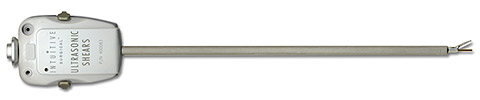
\includegraphics[width=\linewidth]{Endowrist1.jpg}
		\caption{An Endowrist.}
		\label{fig:phantom1}
	\end{subfigure}
	\begin{subfigure}{.45\textwidth}
		\centering
		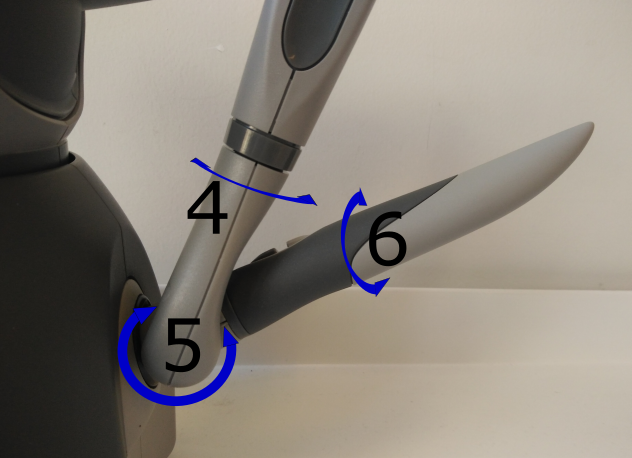
\includegraphics[width=\linewidth]{haptick2.png}
		\caption{Overview of the Phantom omni's last three joint}
		\label{fig:phantom2}
	\end{subfigure}
\caption{Overview of all the Phantom omni's joints\citep{phantom_omni}}
\label{fig:phantom_omni}
\end{figure}
